\documentclass[]{IEEEtran}
%\usepackage{times}
%\usepackage{float}
%\usepackage{geometry}
%\usepackage{fancyhdr}
\usepackage{amsmath}
%\usepackage{array}
\usepackage[pdftex]{graphicx}
\usepackage[font=small, labelfont=bf, justification=centering]{caption}
\usepackage{subcaption}
\usepackage[hidelinks]{hyperref}
\usepackage[english]{babel}
\usepackage{lipsum}
\usepackage{tcolorbox}
\usepackage{titlesec}

%\setcounter{secnumdepth}{2}

%\titleformat{\paragraph}
%{\normalfont\normalsize\bfseries}{\theparagraph}{1em}{}
%\titlespacing*{\paragraph}
%{0pt}{3.25ex plus 1ex minus .2ex}{1.5ex plus .2ex}

\graphicspath{{Images/}}
\bibliographystyle{IEEEtran}

\title{Sentiment Analysis of Tweets to Airlines} 
\author{Rhys Evans (i6150369) and Parth Shrivastava (i6170757)}

\date{Maastricht University  \\[2ex]
    \today
}
\begin{document}

\maketitle

\begin{abstract}
    This report seeks to analyze the sentiment analysis of tweets to six different airline companies.
    The tweets will be classified as positive, neutral, or negative using a training set, a validation set, and a test set.
    Different type of classifiers will be used to conduct tests on sentiment accuracy.
\end{abstract}

\section{Introduction}
We want to conduct sentiment classification of tweets to airlines to determine
whether they are positive (reviews), negative (complaints), or neutral
(statements). This problem is interesting from a business perspective because it is useful to
know which airline has better reviews. Using natural language processing allows
businesses to analyze public opinion through tweets without having to conduct
formal surveys. They can then use this information to drive business decisions
because they will have an insight into what customers think of them and into what
customers think of their competition.

\subsection{Dataset}
The dataset used contains tweets from February 16th to February 24th 2015. The tweets were directed at six
major airlines in the United States. The tweets are classified as either positive,
negative, or neutral. The dataset is called “Airline Twitter sentiment” and is taken
from Figure Eight Inc. \cite{dataset}. 
According to the source, “Twitter data was scraped from February of 2015
and contributors were asked to first classify positive, negative, and neutral
tweets, followed by categorizing negative reasons (such as “late flight” or “rude
service”)”. However, we cannot apply this approach because we do not have the means to survey
contributors and ask them to classify the sentiment of 14640 tweets.

\subsection{Research Question and Hypothesis}
We want to determine which classifier yields the highest accuracy, precision, and recall. We believe that Logistic Regression will be the best classifier because it gives a higher weight for words with a higher chance of affecting the sentiment. This should improve it's accuracy because in tweets and reviews, the words are not independent. They are all dependent on each other to compose a coherent thought. With logistic regression, this is taken into account.

\section{Approach (Bag of Words Representation)}
We approached this problem with Bag of Words. In BOW, the tweets are first cleaned by removing stop-words, which don't have a significant impact on the resulting sentiment of the tweet. The clean tweets are then stored in a vectorized bag of words form. They are then sorted by sentiment by quantifying the tweets: if positive then 1, if negative then -1, if neutral then 0.

\section{Classifiers}
We used a portion of the pre-classified data set to train our approaches. SkLearn was used to implement these classifiers \cite{scikit-learn}.

\subsection{Logistic Regression}
This works by using a linear weighted sum, by assigning different weights to different words in the tweets (higher weights for words which have a higher chance of affecting the resulting sentiment).

\subsection{Gaussian Na{\"i}ve Bayes}
We can use Bayes classifiers with the presence of n-grams and part-of-speech
distribution information, as done in “Twitter as a Corpus for Sentiment Analysis
and Opinion Mining” from Universit{\'e} de Paris-Sud \cite{pak2010twitter}.
It basically makes use of the Bayes Theorem (for a Gaussian distribution) and finds probability of a sentiment given the data(tweet).

\subsection{Random Forest Method}
Another method that has been used in the past is the random forest
method. This classifier was implemented in “Sentiment analysis using product review data” the Journal of Big Data \cite{fang2015sentiment}. In simple terms, the "random forest [classifier] builds multiple decision trees and merges them together to get a more accurate and stable prediction" \cite{TheRando29}. It is an ensemble of Decision Trees that have been trained with the Bootstrap Aggregation method \cite{Brownlee}.

\section{Tests}
We compared the accuracies of different classifiers 
and then conducted significance tests on those accuracies to determine whether
different approaches were more statistically significant than other approaches. These
statistical tests are useful because they can tell us if our model prediction is sufficiently good.

\subsection{Setup}
The training set and test set were split up in such a way that the latest tweets were used as test set, and all the prior tweets as training, so that this way we use our models to "predict" future tweets based on past ones rather than the other way. Tweets from February 16th to February 22nd were used as training data and tweets from February 23rd and 24th were used to test. The tweets used in the test remained constant throughout our tests. The parameters we varied in our experiments were test-size (which tells us how much proportion of data will be split for testing+validation vs training, so the smaller the value, higher the comparative training) and random-state (which randomizes different portions of the data for training/validation).

\section{Experimental Result Analysis}
In figures \ref{rs1}, \ref{rs2}, and \ref{rs3} (which randomize different parts of the data as training/validation), Logistic Regression consistently outperforms Random Forest and Gaussian Na{\"i}ve Bayes, with Gaussian Na{\"i}ve Bayes being the worst of all 3. This is most likely due to the fact that Gaussian Na{\"i}ve Bayes assumes that each feature (word) in a tweet is independent, when in reality, this is not always the case. This big assumption gives it a much lower accuracy. Logistic regression outperforms the other 2 classifiers because it uses a linear combination of the features (words) by assigning higher weights to words which have a higher (maximum) likelihood of affecting a sentiment. It also performs slightly better than Random Forest because Random Forest makes use of decision trees, which, without pruning, make it more prone to overfitting than Logistic Regression as it can scale up to be very complex. Random Forest decision trees would work much better if the task was a high multi-classification with many output class types/labels (in our case it is trinary, i.e, -1,0,1).

\begin{figure}[ht]
    \centering
    \begin{minipage}{0.5\textwidth}
        \centering
        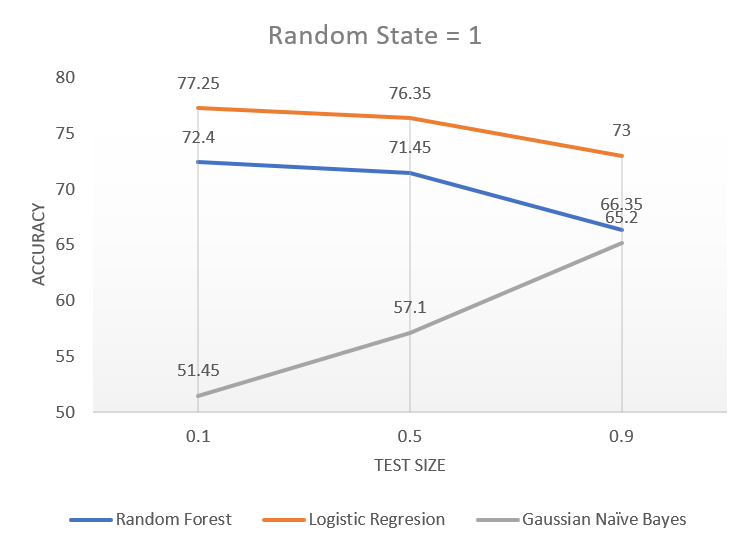
\includegraphics[width=0.9\textwidth]{RS1.png}
        \caption{Classifier performances with random state = 1 \label{rs1}}
    \end{minipage}\hfill
    \end{figure}
\begin{figure}[ht]
    \begin{minipage}{0.5\textwidth}
        \centering
        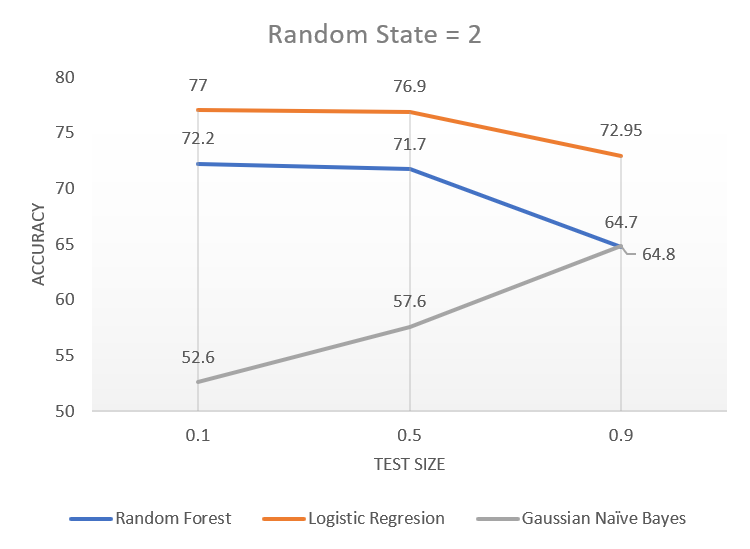
\includegraphics[width=0.9\textwidth]{RS2.png}
        \caption{Classifier performances with random state = 2 \label{rs2}}
    \end{minipage}\hfill
    \end{figure}
\begin{figure}[ht]
    \begin{minipage}{0.5\textwidth}
        \centering
        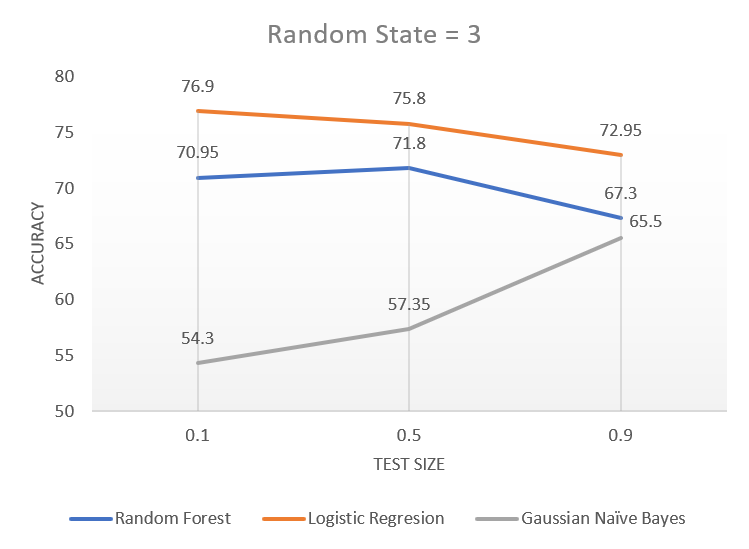
\includegraphics[width=0.9\textwidth]{RS3.png}
        \caption{Classifier performances with random state = 3 \label{rs3}}
    \end{minipage}\hfill
\end{figure}


Another curious thing to note is that the more we train vs validate (i.e, the less we overfit), the better both Logistic Regression and Random Forest work. This is because more overfitting makes it more specific to a certain kind of data, which is not good training for real-world test data. On the other hand, the more we overfit, the better Gaussian Na{\"i}ve Bayes performs. This is because with a larger training (vs validation) set, there is a higher chance of coming across features (words) with a higher dependence on each other, which would be considered independent by this classifier. In other words, Gaussian Na{\"i}ve Bayes gets 'exposed' for its na{\"i}vety of assuming feature independence the more we train. In general it works better for smaller datasets as it is less prone to overfitting.


We also conducted P/R/F1 tests for further evaluation. Our precision, recall, and F1 tests all supported our previous findings that Logistic Regression was the most accurate classifier and that Gaussian Na{\"i}ve Bayes was the least accurate. For these tests, we used the metrics package provided through SKLearn \cite{scikit-learn}. Our recall tests determined the percentage of correct items that were selected, our precision tests determined the percentage of selected items that were correct, and our F1 test assessed the P/R
tradeoff. We were unable to compute the Area Under the Receiver Operating Characteristic curve (AUROC) from prediction scores because our dataset is not binary and AUROC is restricted to the binary classification task.

\begin{figure}[ht]
    \centering
    \begin{minipage}{0.5\textwidth}
        \centering
        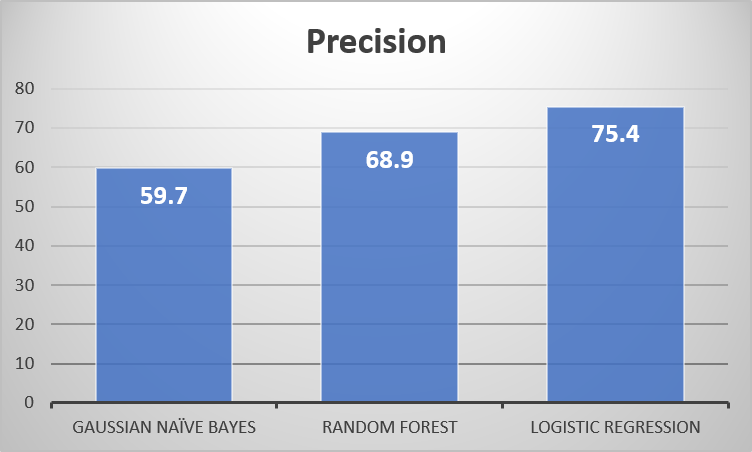
\includegraphics[width=0.9\textwidth]{Precision.png}
        \caption{Precision performance with fixes test size (0.1) and random state (1) \label{precision}}
    \end{minipage}\hfill
    \end{figure}
\begin{figure}[ht]
    \begin{minipage}{0.5\textwidth}
        \centering
        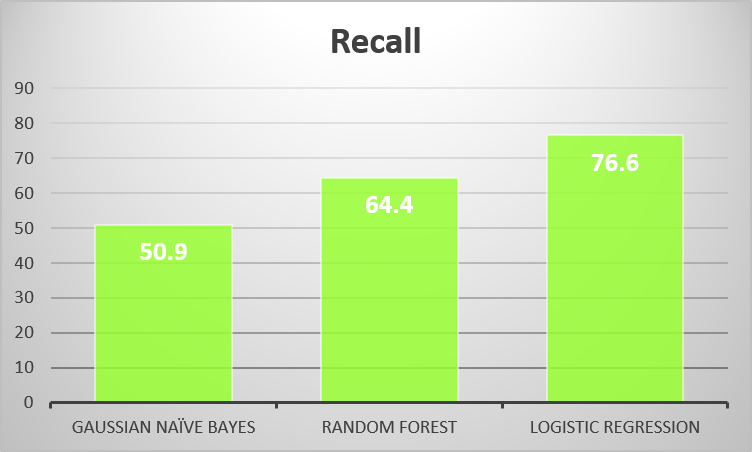
\includegraphics[width=0.9\textwidth]{Recall.png}
        \caption{Recall performance with fixes test size (0.1) and random state (1) \label{recall}}
    \end{minipage}\hfill
    \end{figure}
\begin{figure}[ht]
    \begin{minipage}{0.5\textwidth}
        \centering
        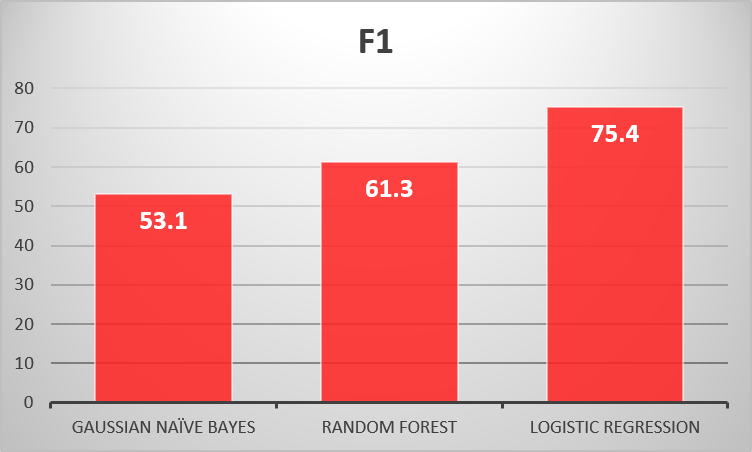
\includegraphics[width=0.9\textwidth]{F1.png}
        \caption{F1 performance with fixes test size (0.1) and random state (1) \label{f1}}
    \end{minipage}\hfill
\end{figure}

\section{Interesting Tests to look At}
One interesting question to research could be how a certain airline company correlates to a certain sentiment. However, it would be necessary to keep in mind that this could have biases based on the context of the airline companies over the internet (if they are used in a positive/negative/neutral reference). Another research possibility would be to look at significance tests to determine how significantly better a given classifier performs etc.

\section{Conclusions}
Many different factors affect which classifier is superior. It depends on factors such as the task at hand, how dependent the dataset is, how large it is, how much of it classified, and what type of classification task it is. Airline sentiment analysis is an interesting task because airline companies are constantly look to better their selves to compete with fellow airlines. This same competitive business paradigm can also be applied to many different fields including hotel ratings, agency ratings, movie rating, and many more. There are countless situations where such data is provided in the form of text (not numbers), and Natural Language Processing combined with Machine Learning is able to give an insight into what's working well and what isn't, and to find key patterns to give an edge to maximize performance.


\bibliography{nlp}

\end{document}      